\section{Background}
\label{sec:background}
This section will briefly mention the background of this research, and will give a summary of the ADRIAN protocol. It will also detail the components of the ADRIAN protocol that are relevant to this research.

\subsection{ADRIAN Protocol}
\label{ssec:adrian}

As mentioned in the introduction, this research builds upon the earlier work of Mann and Smolka \cite{mann2023ADRIAN}. They propose a protocol, called \ADRIAN (or ADRIAN for short), which has the core objective to identify and mitigate risks in distributed systems, leveraging a decentralized and adaptive approach. Unlike conventional security frameworks that rely on a centralized authority to oversee system security, ADRIAN empowers autonomous software agents to collaboratively assess and address security risks. An abstract representation of the ADRIAN approach is shown in Figure \ref{fig:adrian-architecture}.

\begin{figure}
    \centering
    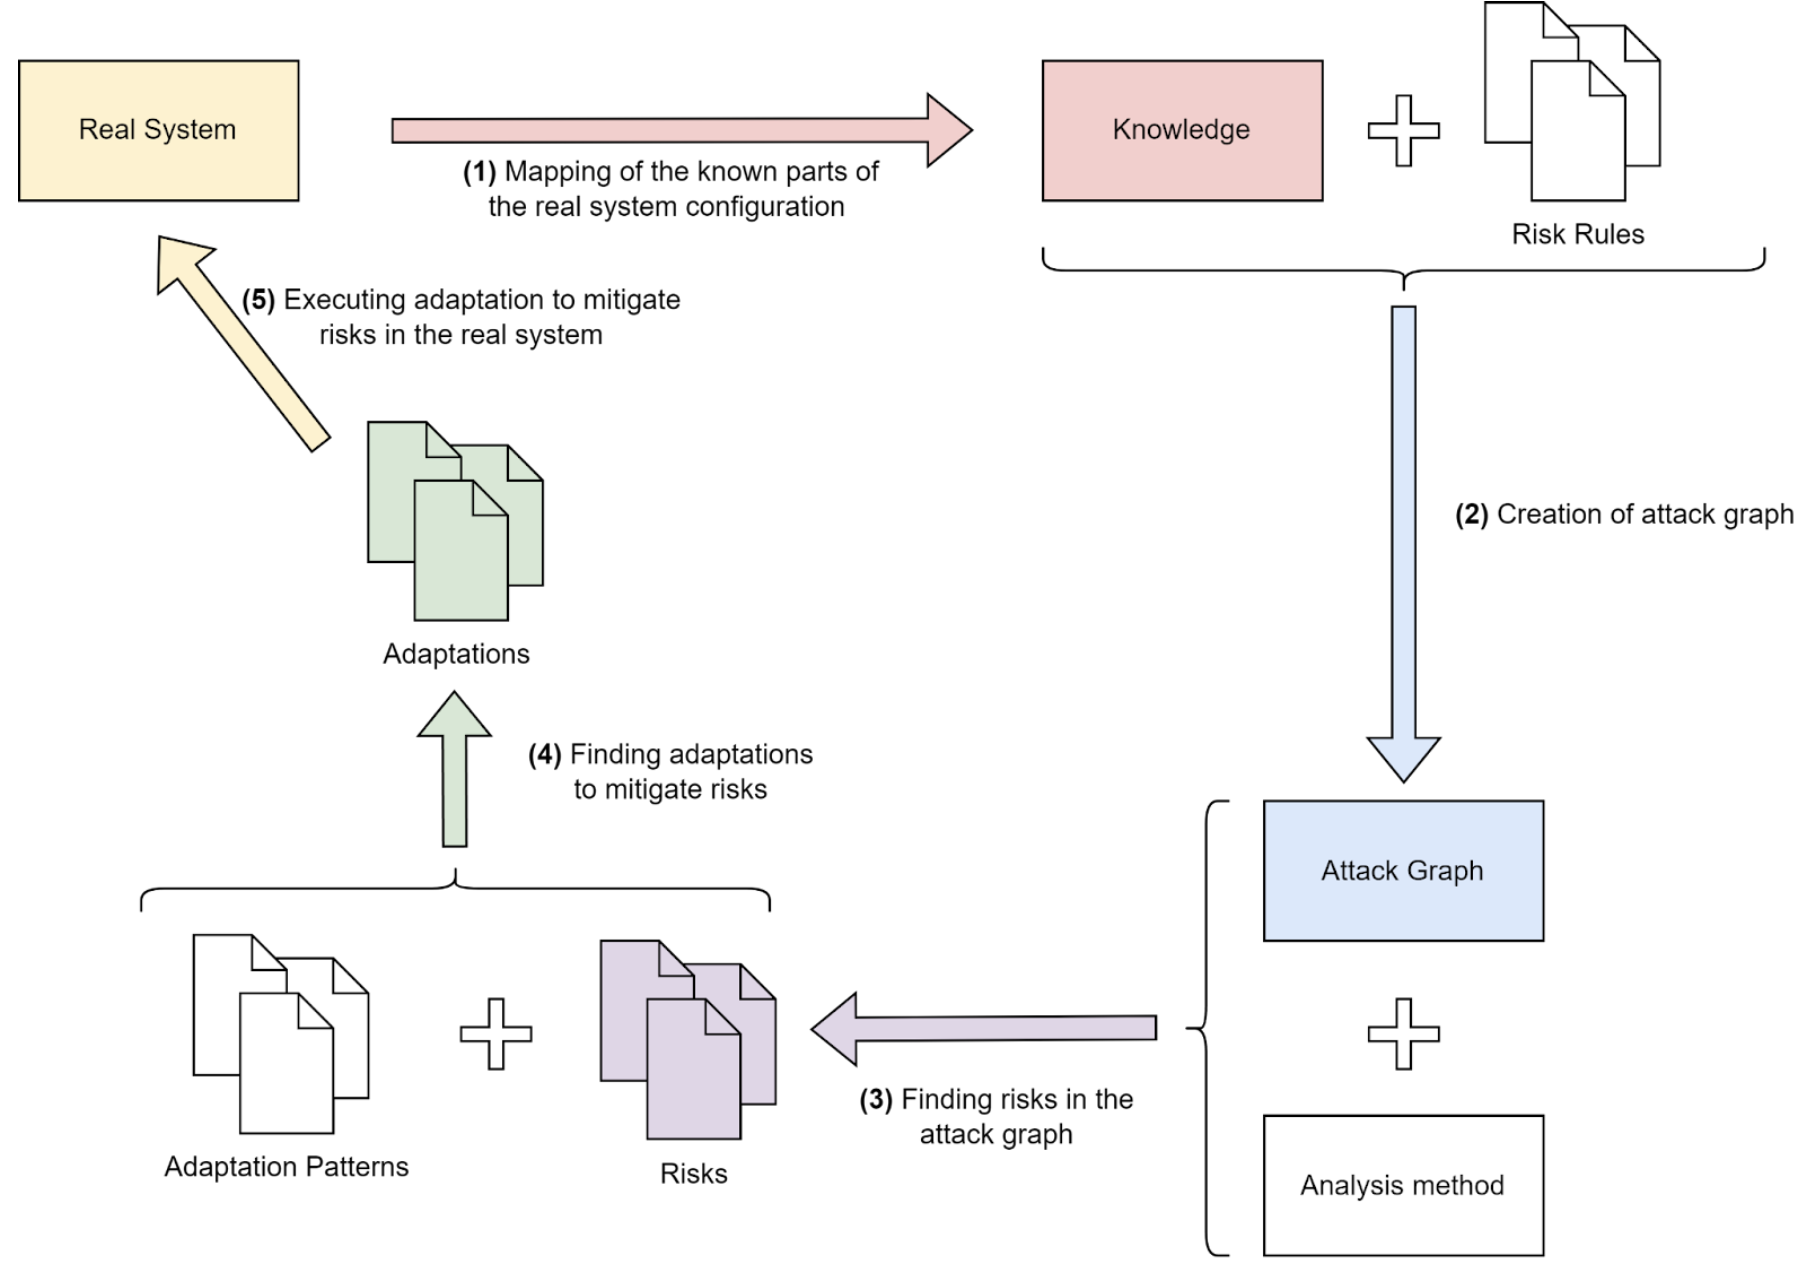
\includegraphics[width=0.8\textwidth]{content/adrian-architecture.png}
    \caption{The abstract representation of the ADRIAN approach. It shows how the different components interact with each other. This figure has been sourced from the ADRIAN concept by Mann and Smolka \cite{mann2023ADRIAN}.}
    \label{fig:adrian-architecture}
\end{figure}

In the ADRIAN protocol, agents are deployed across the infrastructure nodes of a network. These agents are responsible for monitoring the state of the node they are deployed on, specifically the properties of said node. These properties could range from firewall settings to OS and Firmware versions running on the node. Agents also know about the software that is deployed on their infrastructure node and its properties, such as SDK and software library versions, and if data is encrypted on disk. This information is stored by the agent in a localized \emph{knowledge base}. Knowledge about each node, and it's software, is then exchanged between agents. This exchange will slowly propagate the knowledge throughout the network, allowing agents to have a more complete view of the network.

\vspace{0.5em}
To identify risks in a network an agent uses a set of \emph{risk rules}. These risk rules are based on known vulnerabilities, which are registered in the CVE list. They denote the probability of an attacker compromising the node/software. The definition of the risk rules that are implemented are detailed in Section \ref{ssec:risk-rules-adaptaions}.
These risk rules are then applied to the knowledge base to create \emph{attack graphs}, which are used to reason about the risk of a network. These attack graphs serve as a dynamic representation of the network's current status, where each node is represented as a vertex. Each edge (\emph{n1->n2}) represents the risk that an attacker that can compromise \emph{n1}, also manages to compromise \emph{n2}. It is important to note that the attack graph is not an exact reflection of the real network; rather, it is a model derived from local observations and knowledge shared among agents. 
Note that sometimes vulnerabilities and risks are not yet registered as CVEs, but could exist in the real infrastructure. This means that the attack graph is not a 100\% accurate representation of the real world network, as it is not aware of these vulnerabilities. This is a problem, as it could lead to false negatives. However, this is a problem that is not unique to the ADRIAN protocol, as it is also present in other risk detection systems.

\comment{Zoltan}{Critical software component is not explained yet.}
\comment{Zoltan}{Risk report is not explained yet.}
\comment{Zoltan}{Auction is not explainted yet.}
From the attack graph, agents can derive a set of \emph{critical paths} that represent a path to a critical software component. These critical paths are then used to determine the risk of a network and the potential damage that could be done which results in a \emph{risk report}. One of these risk reports is selected and will be auctioned off to the agents in the network. In order to calculate the potential damage of a risk, the agent will combine all the probabilities of each individual edge of the attack graph along the critical path, using the following formula:

\[p = 1 - \prod_{k=1}^{R}(1-p_{k}) \]

Where $R$ is the number of all risks rules that lead to a risk edge between nodes a and b. $p_{k}$ is the probability of one of the risk rules from $R$. This formula gives us a single probability $p$ per edge. Calculating the product of all probabilities $p$ along the critical path, gets the final probability. This final probability is then multiplied with the critical software components damage (predetermined) to get the expected damage of the risk.

\vspace{0.5em}
The auctioning system is a mechanism that lets agents invite their peers to participate in the risk mitigation process. Once an agent has started an auction, other agents are invited to participate. These participating agents receive the risk report and attack graph as calculated by the initiating agent. Through a set of \emph{adaptation patterns}, agents can find multiple proposed solutions to reduce the potential damage of the risk report. These adaptation patterns are based on the risk rules, and describe possible adaptations that can be performed to mitigate the risk.
Each participating agent tries to find and select a proposal that mitigate the risk. This proposal is then sent back to the auctioneer agent, which will accumulate all proposals and select the proposal that is most beneficial to the network. The selected proposal is then executed by the agent that proposed it, and the network is updated accordingly.
